\refstepcounter{figure}
\noindent Figure \thefigure\ shows PDR comparison under simulation variation.

\begin{center}
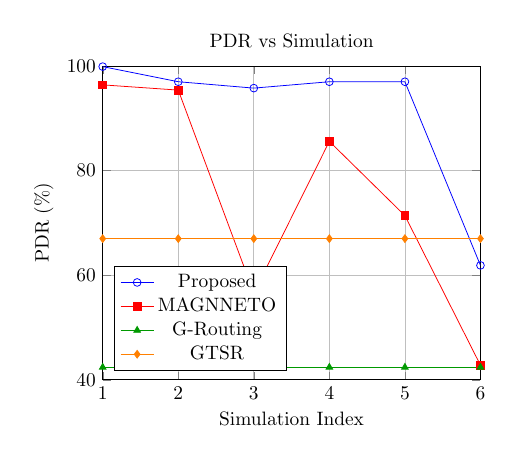
\begin{tikzpicture}[scale=0.7]
\begin{axis}[
title={PDR vs Simulation},
xlabel={Simulation Index}, ylabel={PDR (\%)},
xmin=1, xmax=6, ymin=40, ymax=100,
legend pos=south west,
xtick={1,2,3,4,5,6},
grid=both
]

\addplot[blue, mark=o] coordinates {(1,99.89) (2,97) (3,95.78) (4,97) (5,97) (6,61.89)};
\addplot[red, mark=square*] coordinates {(1,96.4) (2,95.4) (3,56.6) (4,85.6) (5,71.4) (6,42.8)};
\addplot[green!60!black, mark=triangle*] coordinates {(1,42.4) (2,42.4) (3,42.4) (4,42.4) (5,42.4) (6,42.4)};
\addplot[orange, mark=diamond*] coordinates {(1,67) (2,67) (3,67) (4,67) (5,67) (6,67)};

\legend{Proposed, MAGNNETO, G-Routing, GTSR}

\end{axis}
\end{tikzpicture}

\textbf{Figure \thefigure: PDR vs Simulation}
\end{center}